\subsection{Algorytm Kruskala}

Algorytm Kruskala podobnie jak algorytm Prima jest oparty na tworzeniu minimalnego drzewa rozpinającego. Algorytm traktuje ściany między polami labiryntu jako potencjalne krawędzie (przejścia w labiryncie). Działanie algorytmu w kontekście labiryntu przebiega następująco:

\begin{enumerate}
    \item Na początku tworzona jest plansza, w której wszystkie pola są oznaczone jako przejśćia.

    \item Tworzony jest zbiór rozłącznych zbiorów \textit{Disjoint Set}, w którym każda komórka należy do własnego zbioru — oznacza to, że na początku żadna komórka nie jest połączona z inną.

    Struktura \textit{Disjoint Set} reprezentuje rozłączne zbiory elementów za pomocą drzew. Na początku każdy element tworzy pojedynczy, jednoelementowy zbiór, którego reprezentantem jest korzeń drzewa.

    Kluczową operacją na tej strukturze jest \textit{Union}, która łączy dwa zbiory, tworząc jedno drzewo, w którym korzeń jednego zbioru staje się potomkiem korzenia drugiego. W ten sposób zbiory są scalane.

    Schematyczne przedstawienie scalania zbiorów znajduje się na Rysunku \ref{fig:disjoint_set}.

    \begin{figure}[ht]
    \centering
    \begin{subfigure}{0.24\textwidth}
        \centering
        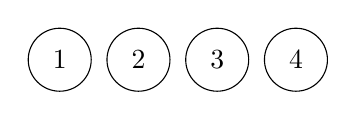
\begin{tikzpicture}[scale=1, every node/.style={circle,draw,minimum size=8mm}]
            \node (n0) at (0,0) {1};
            \node (n1) at (1,0) {2};
            \node (n3) at (2,0) {3};
            \node (n4) at (3,0) {4};
        \end{tikzpicture}
        \caption{Krok 1}
        \label{fig:disjoint_set_a}
    \end{subfigure}
    \begin{subfigure}{0.24\textwidth}
        \centering
        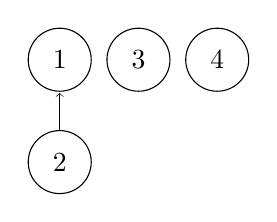
\begin{tikzpicture}[scale=1, every node/.style={circle,draw,minimum size=8mm}]
            \node (n0) at (0,1.3) {1};
            \node (n1) at (0,0) {2};
            \node (n2) at (1,1.3) {3};
            \node (n3) at (2,1.3) {4};
            \draw[->, very thin, black] (0,0.4) -- (0,0.88);
        \end{tikzpicture}
        \caption{Krok 2}
        \label{fig:disjoint_set_b}
    \end{subfigure}
    \begin{subfigure}{0.24\textwidth}
        \centering
        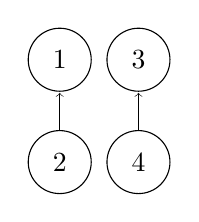
\begin{tikzpicture}[scale=1, every node/.style={circle,draw,minimum size=8mm}]
            \node (n0) at (0,1.3) {1};
            \node (n1) at (0,0) {2};
            \node (n2) at (1,1.3) {3};
            \node (n3) at (1,0) {4};
            \draw[->, very thin, black] (0,0.4) -- (0,0.88);
            \draw[->, very thin, black] (1,0.4) -- (1,0.88);
        \end{tikzpicture}
        \caption{Krok 3}
        \label{fig:disjoint_set_c}
    \end{subfigure}
    \hfill
    \begin{subfigure}{0.24\textwidth}
        \centering
        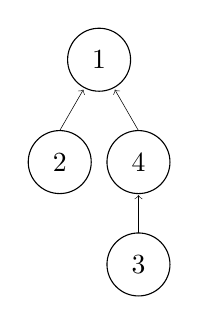
\begin{tikzpicture}[scale=1, every node/.style={circle,draw,minimum size=8mm}]
            \node (n0) at (0.5,2.6) {1};
            \node (n1) at (0,1.3) {2};
            \node (n2) at (1,0) {3};
            \node (n3) at (1,1.3) {4};
            \draw[->, very thin, black] (0,1.7) -- (0.3,2.22);
            \draw[->, very thin, black] (1,1.7) -- (0.7,2.22);
            \draw[->, very thin, black] (1,0.4) -- (1,0.88);
        \end{tikzpicture}
        \caption{Krok 4}
        \label{fig:disjoint_set_d}
    \end{subfigure}
    \caption{Kolejne kroki scalania zbioru}
    \label{fig:disjoint_set}
\end{figure}
%https://cp-algorithms.com/data_structures/disjoint_set_union.html

    \item Zbierane są wszystkie możliwe krawędzie, czyli miejsca między dwiema bezpośrednio sąsiadującymi komórkami, które można potencjalnie zamienić na ściany. Następnie są one tasowane w losowej kolejności. W odróżnieniu od algorytmu Prima, za sąsiadujące uznaje się tutaj pola przylegające bezpośrednio.

    \item Iterujemy po każdej ścianie ze zbioru:
    \begin{enumerate}
        \item Dla danej ściany sprawdzane są dwie komórki, które ta ściana oddziela.
        \item Jeśli te komórki należą do różnych zbiorów (nie są jeszcze połączone), to:
        \begin{enumerate}
            \item Usuwana jest ściana między nimi - tworzy się przejście.
            \item Obie komórki zostają połączone w jednym zbiorze.
        \end{enumerate}
        \item Jeśli komórki są już w tym samym zbiorze (czyli istnieje już droga między nimi), ściana nie jest usuwana — zapobiega to tworzeniu cykli.
    \end{enumerate}

    \item Proces trwa do momentu, gdy wszystkie komórki zostaną połączone w jeden zbiór — czyli zostanie utworzone jedno spójne drzewo bez cykli.
\end{enumerate}